\documentclass[a4paper,11pt,uplatex]{jsarticle}
\usepackage{myreport}
\renewcommand{\thesection}{3-\arabic{section}}
\title{Chapter3}
\author{20B01392 松本侑真}
\date{\today}
\begin{document}
\maketitle
\begin{abstract}

\end{abstract}
\tableofcontents
\newpage

\setcounter{section}{5}
\section{Yukawa Theory of Nuclear Interaction}
湯川が1934年に提唱した中間子の交換というアイデアは、以前の章の対称的な議論を通して得られたものを超えて、
核子間相互作用を調べるのには良いスタート地点である。
湯川の描像では、2つの核子間の相互作用は中間子の交換によって仲介される。
クォークの構造が根底にある、ハドロンの量子的な繋がりを率直に描いてはいないが、
その理論は中間子と核子間相互作用の強さのように、核子の相互作用を他のいろいろなハドロン原子の過程に結びつけることができる。
より実証的なレベルでは、湯川のアイデアは核子のポテンシャルの距離依存性の合理的なモデルを提供してくれる。
そのような表現は、例えば、半経験的なアプローチ方法として使えるかもしれない。
本章における焦点は、主に中間子交換のアイデアの起源そのものである。
応用については最終章に残すことにして、核子-核子散乱から提供される実験的な情報を最初に確認する。

ボソンの交換に基づくポテンシャルの適切な導出は、今扱っている範疇を超えている、相対論的な場の量子論を扱う必要がある。
しかしながら、そのエッセンスは古典的な電気力学とのアナロジーを考えることで得られる。
湧き出しのない場所の静電ポテンシャル$\phi(\bm{r})$は、ラプラス方程式の解となっている:
\begin{equation}
  \laplacian\phi(\bm{r})=0\;。
  \label{eq:laplas}
\end{equation}
電荷$q$の点電荷が原点に存在しているとき、方程式は
\begin{equation}
  \laplacian\phi(\bm{r})=-\qty[\frac{1}{4\pi\varepsilon_0}]4\pi q\delta(\bm{r})
  \label{eq:poisson}
\end{equation}
となる。この解として、良く知られているクーロンポテンシャルが得られる:
\begin{equation}
  \phi(\bm{r})=\qty[\frac{1}{4\pi\varepsilon_0}]\frac{q}{r}\;。
  \label{eq:3-59}
\end{equation}
電磁場が量子化されるとき、場の量子として光子が出現し、電荷は場の源となる。(どういう意味ですか?)
\vskip\baselineskip
\begin{tcolorbox}[
    colback = white,
    colframe = green!35!black,
    fonttitle = \bfseries]
  \begin{theorem}[Poisson方程式の解]
    一般に、Poisson方程式は
    \begin{equation}
      \laplacian u(\bm{r})=-f(\bm{r})
    \end{equation}
    と表される。このとき、解は
    \begin{equation}
      u(\bm{r})=\frac{1}{4\pi}\iiint d^3\bm{r}'\,\frac{f(\bm{r}')}{\abs{\bm{r}-\bm{r}'}}
    \end{equation}
    である。
  \end{theorem}
\end{tcolorbox}
核力は電磁気的な力とは異なる点がいくつかある。
恐らく最も重要な点は、それが短距離力ということであり、次章でそれを支持する証拠を確認する。
今は、短距離の核ポテンシャルに対する場の量子論における類似物である
式\eqref{eq:poisson}と似た式の問題を主に考えることにする。
考える式は、相対論的極限でも成立するために、ローレンツ共変でなければならない。
シュレディンガー方程式は非相対論的極限でのみ適用されるため、このルールを満たしていない。
核子を交換している場の量子はボソンでなければならない。なぜなら、ボソンのみが単体で生成消滅することが可能だからである。
フェルミオンは一方で、その反粒子とともに生成消滅する。ディラック方程式はスピン$1/2$の粒子(言い換えれば、フェルミオン)を記述する方程式であるため不適当である。
第一候補としては、クライン・ゴルドン方程式が残されている。

相対論的なエネルギー運動量関係は、
\begin{equation}
  E^2=p^2c^2+m^2c^4
\end{equation}
で与えられる。
エネルギー$E$を演算子$i\hbar(\pdv*{t})$に、運動量$\bm{p}$を演算子$-i\hbar\grad$に置き換えることで、
非相対論的な量子力学を得たときと同様の方法で量子化することができる:
\begin{equation}
  -\hbar^2\pdv[2]{t}\phi(\bm{r}) = \qty(-\hbar^2c^2\laplacian + m^2c^4)\phi(\bm{r})\;。
\end{equation}
ここで、$m$は場の量子の質量とする。両辺に$(\hbar c)^2$をかけて整理すると、良く知られたクライン・ゴルドン方程式を得る:
\begin{equation}
  \qty(\laplacian - \frac{1}{c^2}\pdv[2]{t})\phi(\bm{r}) = \frac{m^2c^2}{\hbar^2}\phi(\bm{r})\;。
  \label{eq:3-61}
\end{equation}
これは、場の量子のソース項はまだ含まれていないため、式\eqref{eq:laplas}のアナロジーにすぎない。
この点は、場の量子の質量$m$をゼロにして、時間依存性を無視することでさらに実証されるかもしれない。
その結果は、式\eqref{eq:laplas}と同じである。

湧き出しを含めるためには、式\eqref{eq:3-61}にソース項を追加して、ポアソン方程式\eqref{eq:poisson}に相当するものを求める必要がある。
簡単化のため、静止限界(static limit)のみを考えて、時間微分を含む項を無視する。
原点に強さが$g$の点源があるとき、
\begin{equation}
  \laplacian\phi(\bm{r}) = \frac{m^2c^2}{\hbar^2}\phi(\bm{r}) - g\delta(\bm{r})
  \label{eq:3-69}
\end{equation}
を得る。この式の解
\begin{equation}
  \phi(\bm{r})=\frac{g}{4\pi r}e^{-mcr/\hbar}
\end{equation}
は、湯川ポテンシャルの形として良く知られており、$m=0,\,g=\qty[(4\pi\varepsilon_0)^{-1}]4\pi q$とすることで、
式\eqref{eq:3-59}に帰着できる。
一方で、もし場の量子に有限の質量があると、ポテンシャルの強さが$r_0=\hbar/mc$で$1/e$倍に落ちることがわかる。
$r_0$は、質量$m$のボソンが仲介する力の範囲の尺度として捉えることができる。パイ中間子($m\sim \SI{140}{MeV/c^2}$)では、
$r_0$の値はおよそ\SI{1.4}{fm}である。後で見るように、1つのパイ中間子の交換は、核力ポテンシャルの長距離部分をよく表現している。

\vskip\baselineskip
\begin{tcolorbox}[
    colback = white,
    colframe = green!35!black,
    fonttitle = \bfseries]
  \begin{theorem}[湯川ポテンシャルの導出]
    点源がある場合のクライン・ゴルドン方程式
    \begin{equation}
      \laplacian\phi(\bm{r}) = \frac{m^2c^2}{\hbar^2}\phi(\bm{r}) - g\delta(\bm{r})
      \label{eq:3-611}
    \end{equation}
    のFourier変換を考える。
    以下では、関数$f(\bm{r})$のFourier変換を
    \begin{equation}
      \mathcal{F}[f]\coloneqq \frac{1}{(2\pi)^3}\int_{-\infty}^{\infty} d^3\bm{r} f(\bm{r})e^{-i\bm{k}\cdot\bm{r}}
    \end{equation}
    と定義する。
    $\mathcal{F}[\laplacian f] = -\abs{\bm{k}}^2\mathcal{F}[f]$
    となることは部分積分から容易に示すことができ、式\eqref{eq:3-611}の両辺をFourier変換すると
    \begin{equation}
      \mathcal{F}[\phi] = \frac{g}{(2\pi)^3}\frac{1}{k^2+m^2c^2/\hbar^2}
    \end{equation}
    となる。したがって、逆Fourier変換は以下のようになる:
    \begin{equation}
      \phi(\bm{r}) = \frac{g}{(2\pi)^3}\int_0^\infty dk\frac{k^2}{k^2+m^2c^2/\hbar^2}\int_{-1}^{1}d(\cos\theta) e^{ikr\cos\theta}\int_{0}^{2\pi}d\varphi \,。
    \end{equation}
    ここで、
    \begin{equation}
      \int_{-1}^{1}d(\cos\theta) e^{ikr\cos\theta} = \frac{1}{ikr}\qty[e^{ikr} - e^{-ikr}]
    \end{equation}
    となり、第二項目は第一項目で$k\to-k$とした場合に対応しているため、
    \begin{equation}
      \phi(\bm{r}) = \frac{g}{(2\pi)^2ir}\int_{-\infty}^{\infty}dk\frac{ke^{ikr}}{k^2+m^2c^2/\hbar^2}
    \end{equation}
    となる。$r>0$であるため、複素平面の上半分を通る半径$R$の半円経路を考えると、$R\to\infty$で半円上での積分は$0$に収束する。したがって、
    \begin{equation}
      \phi(\bm{r}) = \left.\frac{g}{2\pi r}\frac{ke^{ikr}}{(k^2+m^2c^2/\hbar^2)'}\right|_{k=imc/\hbar} = \frac{g}{4\pi r}e^{-mcr/\hbar}
    \end{equation}
    を得る。
  \end{theorem}
\end{tcolorbox}

\newpage
\section{Nucleon-Nucleon Scattering Phase Shifts}
核子-核子相互作用によるポテンシャルの表式
\begin{align}
  V(r;\,\bm{\sigma}_1,\,\bm{\sigma}_2,\,\bm{\tau}_1,\,\bm{\tau}_2) \;=\; &
  V_0(r)+V_\sigma(r)\bm{\sigma}_1\cdot\bm{\sigma}_2 + V_\tau(r)\bm{\tau}_1\cdot\bm{\tau}_2
  + V_{\sigma\tau}(r)\qty(\bm{\sigma}_1\cdot\bm{\sigma}_2)\qty(\bm{\tau}_1\cdot\bm{\tau}_2) \notag                                                    \\
                                                                         & +V_{LS}(r)\bm{L}\cdot\bm{S} +
  V_{LS\tau}(r)\qty(\bm{L}\cdot\bm{S})\qty(\bm{\tau}_1\cdot\bm{\tau}_2) \notag                                                                        \\
                                                                         & +V_{T}(r)S_{12}+V_{T\tau}(r)S_{12}\qty(\bm{\tau}_1\cdot\bm{\tau}_2) \notag \\
                                                                         & +V_Q(r)Q_{12}+V_{Q\tau}(r)Q_{12}\bm{\tau}_1\cdot\bm{\tau}_2 \notag         \\
                                                                         & + V_{PP}(r)\qty(\bm{\sigma}_1\cdot\bm{p})\qty(\bm{\sigma}_2\cdot\bm{p})
  +V_{PP\tau}(r)\qty(\bm{\sigma}_1\cdot\bm{p})\qty(\bm{\sigma}_2\cdot\bm{p})\qty(\bm{\tau}_1\cdot\bm{\tau}_2)
\end{align}
は、重陽子の方法と、二核子系の対称性を用いて得られた。さらなる飛躍のためには追加の実験的な情報が必要であり、ある核子が異なるエネルギーを持つ別の核子から散乱されることでもたらされる。

\subsection*{Nucleon-nucleon scattering}
原理的に、2つの核子を含む4種類の散乱測定が可能である。入射陽子が陽子によって散乱されること($pp$-scattering)は、実験的観点から、4つのうちで最も単純である。
なぜなら、陽子を加速や、水素(陽子)を含む標的の構築が比較的簡単であるためである。中性子散乱では、入射ビームは大まかに2つの源がある。
低エネルギーでは、原子炉中の中性子が使われる。高エネルギーでは、例えば、\ce{^{7}Li}を標的とする$(p,\,n)$反応のように、陽子ビームから作られる中性子を使うことができる。
しかしながら、これらの方法で得られる中性子ビームの強度やエネルギー分解能は、陽子ビームのそれよりもはるかに制限されている。
その結果、中性子散乱は、一般的に、陽子散乱よりも難しい実験である。
陽子標的からの中性子散乱($np$-scattering)と、それに準ずる$pn$散乱は、$T=0$チャンネルでも反応が生じるという点で重要である。
対称的に、$pp-$と$nn-$散乱は2核子系の$T=1$状態の情報しか提供しない。(なぜ?)

$pp-$と$np-$散乱測定に加えて、原理的には$pn-$と$nn-$散乱実験も可能である。ここでは、陽子を標的として使う代わりに、中性子標的が用いられる。
自由な中性子は10分のオーダーで半減期を迎える不安定な粒子である。それゆえ、水素原子が含まれる材料が使われる陽子とは対照的に、
中性子は固定標的として使うことは不可能である。この制限を回避するために、原理的には2つの方法が存在する。
一つ目の方法は、衝突ビーム実験を行うことである。実験室で標的を固定する代わりに、二次的な中性子ビームが用いられ、
固定標的から入射ビームが散乱される代わりに、2粒子のビームが互いに直接向けられる。
散乱は、2つのビーム中の粒子が衝突する際に生じる。実用的には、2つのビームが高強度である実験が必要であるが、現在では中性子の高強度ビームを簡単には使うことができない。

もう一つの方法は、重水素を用いて固定中性子標的をシミュレーションすることである。重水素は中性子と陽子が緩く結合している系であるため、
$pn-$と$nn-$散乱は$pd-$と$nd-$散乱実験を行うことで得られる。重水素標的中の陽子による寄与は、$pp-$と$np-$散乱実験の結果に対応する測定値を引き算することで取り除くことができる。
この手続きは次の場合に正当化される:
\begin{enumerate}
  \item 十分な精度の元で引き算が行われること。これは、対応する陽子標的による散乱データが完璧にもしくは、より正確に得られていることと、
        重水素の結合エネルギーによる効果を満足行く方法で修正されることが必要である。一般に、これら2つのポイントは比較的簡単に達成することができる。

  \item 三体効果が無視できること。核子が重水素と相互作用する際には、全体系は3つの核子から構成される。
        もし基本的な三体力が存在していると、1つの核子が他のもう1つの核子と散乱する場合ではなく、$pd-$と$nd-$散乱中にその寄与が存在する。
        したがって、例えば陽子-重陽子散乱では、$pp-$と$pn-$散乱による寄与を独立なものとして、単純に足し算すれば良いというわけではない。
        先に見たように、これは問題にはならない。なぜなら、三体力はもし存在しても、弱いものだと期待されるためである。
\end{enumerate}

$pn-$と$nn-$散乱から得られる情報は、$np-$と$pp-$散乱から得られるそれと何の違いもないかもしれない。
例えば、$pn-$と$np-$散乱の唯一の違いは中性子と陽子どちらが標的であるかというものである。
時間反転対称性の元では、それら2つは同じ結果を与えるものと期待される。(なぜ時間反転対称性なのか?重心座標系から見ると同じというだけではだめなのか。)

先に見たように、$pp$と$nn$は$T=1$の系である。もし核力が電荷に依存しないならば、$pp-$と$nn-$散乱の結果の違いはクーロン相互作用による寄与のみである。
後者(クーロン相互作用)は良く知られてるため、$pp-$と$nn-$散乱の結果で原理的に、核力相互作用の電荷依存性をテストすることができる。
しかし、$nn-$散乱を用いた実験の正確性は、そのテストを行うにはいまだ不十分である。次章で見るように、比較的簡単に低エネルギーでは正確な実験を行うことができる。

表記を簡単にするため、中性子と陽子の違いを区別する必要がない場合に、$NN$という記号は2核子系を表すことにする。
また、$np$という記号は、それ以上の区別が必要な場合を除き、$np$と$pn$を表す。
さらに、クーロン力による寄与はすでに取り除かれているものとし、そのため議論において無視することにする。

我々の主要な興味は、散乱のデータと$NN-$相互作用ポテンシャルを関連付けることである。
様々なエネルギーと散乱角による測定値のデータが長年溜まってきた。
ポテンシャル$V$を直接的に差なんデータに関連付ける代わりに、実験の情報を$l-$部分波の位相のずれ$\delta_l$に帰着させることがより一般的である。
例として図\ref{fig:3-3}に書かれるように、計算された位相のズレと実験データから得られる位相のズレを比較することで、特定のポテンシャルの良し悪しを判断することが多い。
このような理由から、まずは簡単に$NN-$散乱における部分波解析について調べる。より詳しい議論は\S{B-2}で与えられている。
\begin{figure}[H]
  \centering
  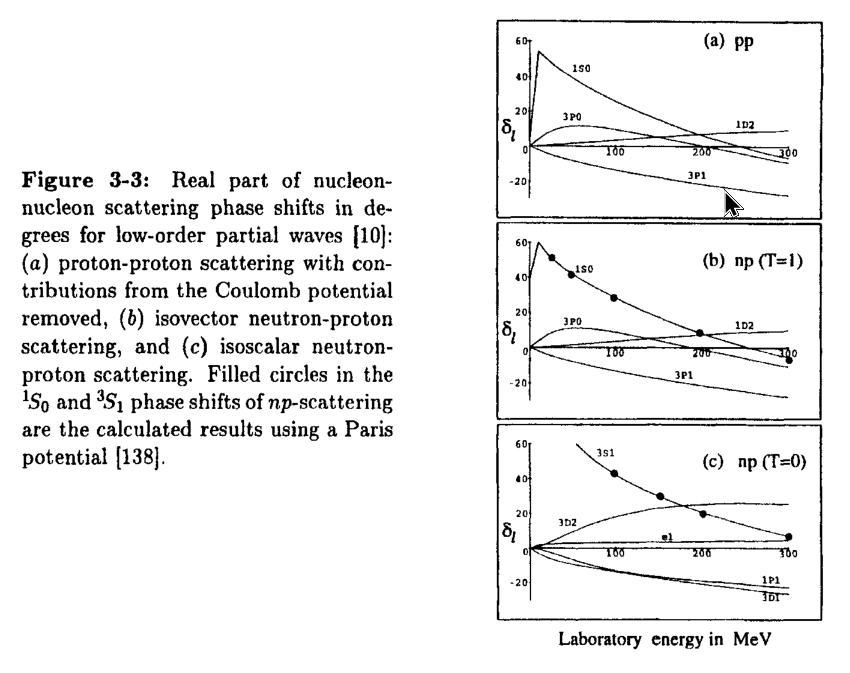
\includegraphics[width=0.8\linewidth]{phaseshift.png}
  \caption{位相のずれの評価}
  \label{fig:3-3}
\end{figure}

\newpage
\subsection*{Scattering cross section}
散乱実験で測定される物理量は、角度$(\theta,\,\phi)$方向の検出器でのカウント回数である。
カウント率は、
\begin{itemize}
  \item 散乱中心から検出器までの立体角
  \item 入射ビームの強度
  \item 反応に巻き込まれた標的核の数
  \item 微分散乱断面積$\dv*{\sigma}{\Omega}$
\end{itemize}
に依存する。主要な興味は$\dv*{\sigma}{\Omega}$であり、散乱角と同様にエネルギーの関数である。

非相対論的極限において、一つの粒子が別の粒子によって散乱される現象は、Shr\"{o}dinger方程式によって記述される。
質量中心において、波動関数は
\begin{equation}
  -\frac{\hbar^2}{2\mu}\laplacian\psi + (V-E)\psi=0
\end{equation}
の解となっている。ここで、$\mu$は2核子系の換算質量である。
主に考えるのは短距離核力(\S{B-5}にクーロン散乱が書かれてある)であり、
その結果、散乱が生じている場所の小さな近傍意外で$V=0$と仮定できる。

$V$がゼロと異なる小さな領域から遠く離れた漸近領域では、波動関数は
\begin{equation}
  \psi(r,\,\theta,\,\phi)\xrightarrow[r\to\infty]{} e^{ikz} + f(\theta,\,\phi)\frac{e^{ikr}}{r}
\end{equation}
の形をしている。ここで、$e^{ikz}$の項は入射平面波であり、反応によって入射波は影響を受けていないことを表している。
散乱された波は$e^{ikr}/r$の球面波で表され、散乱中心から放射状に広がる。$(\theta,\,\phi)$方向へ散乱される確率は
散乱振幅$f(\theta,\,\phi)$で特徴づけられる。簡単にするために、最初は弾性散乱のみを考える。
その結果、2粒子の質量中心から見ると、波数$k$は散乱前後の大きさが等しい。
$(\theta,\,\phi)$方向の微分散乱断面積は式(B-7)で与えられ、散乱振幅の2乗で与えられる:
\begin{equation}
  \dv{\sigma}{\Omega}(\theta,\,\phi) = \abs{f(\theta,\,\phi)}^2\;。
\end{equation}
\begin{figure}[H]
  \centering
  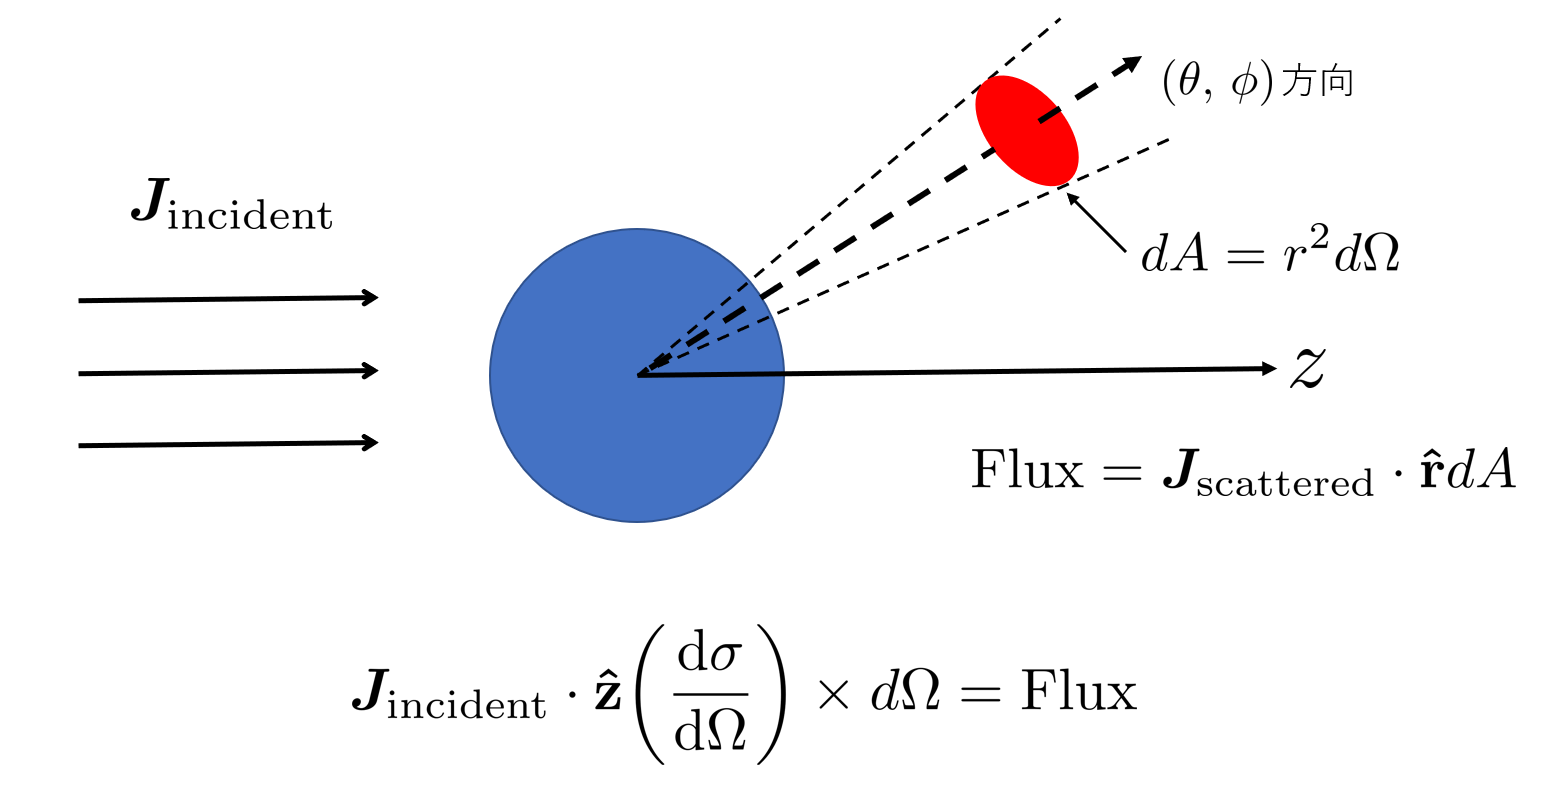
\includegraphics[width=0.8\linewidth]{bibun_sanran_danmenseki.png}
  \caption{微分散乱断面積の図解}
  \label{fig:bibun_sanran}
\end{figure}

図\ref{fig:diagram}にあるように、散乱に関する幾何学は、座標系の原点を散乱の中心として、入射ビームの方向を$z$軸正方向にとる。
入射波の波数ベクトル$\bm{k}$と、散乱波の波数ベクトル$\bm{k}'$は平面を構成し、それは散乱平面となっている。

もし入射ビーム内の核子と標的内の核子が偏極していない場合、すなわち、固有スピンが整列する空間上の特定の方向が存在しない場合、
散乱は$z$軸周りの回転に関して不変である。この場合、断面積は方位角$\phi$に依存せず、微分散乱断面積は$\theta$だけの関数となる。
後に、散乱に関与する1つまたは複数の核子について、内部スピンの向きが検出される場合の一般のケースについて考える。

\begin{figure}[H]
  \centering
  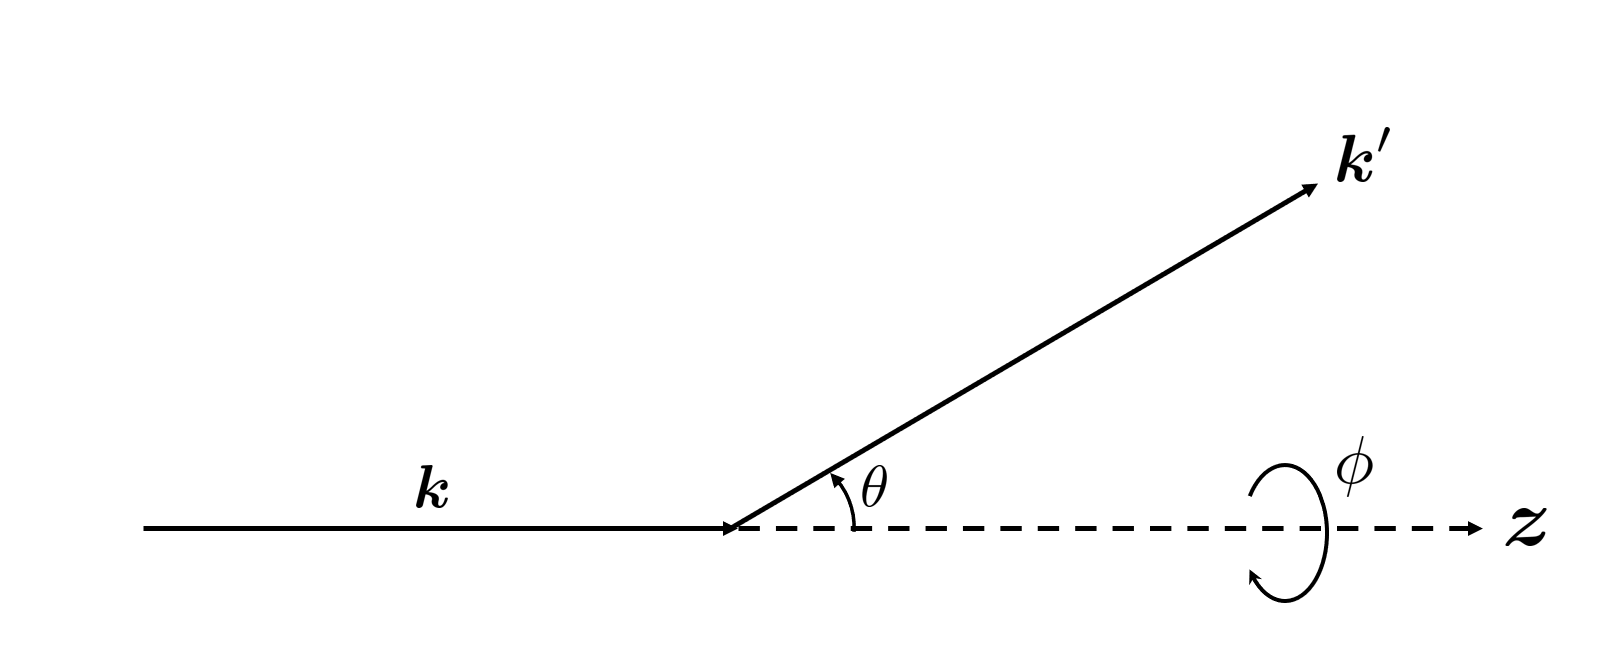
\includegraphics[width=0.6\linewidth]{diagram_scattering.png}
  \caption{散乱前後の波数ベクトルと角度について}
  \label{fig:diagram}
\end{figure}

\subsection*{Partial-wave analysis}
中心力ポテンシャルのため、2つの散乱核子の相対的な角運動量$\bm{l}$は量子化されて観測される。
このような状況において、波動関数をそれぞれが$l$の値で定義される異なる部分波の寄与による和として展開するのが便利である:
\begin{equation}
  \psi(r,\,\theta)=\sum_{l=0}^{\infty} a_lY_{l0}(\theta)R_l(k,\,r)\;。
\end{equation}
ここで、$a_l$は展開係数である。球面調和関数$Y_{lm}(\theta,\,\phi)$において$m=0$のみが現れているのは、
偏極を無視している場合、波動関数は方位角$\phi$に依存しないためである。
波動関数がエネルギーに依存することを強調するため、波数$k$を動径方向の関数$R_l(k,\,r)$に陽に含めている。

$V=0$の自由粒子の場合、動径波動関数は以下のようになる:
\begin{equation}
  R_l(k,\,r)\xrightarrow[]{\text{free}} j_l(kr)\xrightarrow[r\to\infty]{\text{free}} \frac{1}{kr}\sin(kr-l\pi/2)\;。
\end{equation}
ここで、$k=\sqrt{2\mu E}/\hbar$であり、$j_l(\rho)$は$l$次の球ベッセル関数である。
もし、ポテンシャルによって弾性散乱のみが許されているならば、各部分波において、確率密度の流れは保存する。
ポテンシャルによって波動関数に与える唯一の影響は位相の変化である。言い換えると、
\begin{equation}
  R_l(k,\,r)\xrightarrow[r\to\infty]{\text{scatt.}} \frac{1}{kr}\sin(kr-l\pi/2+\delta_l)
\end{equation}
となる。ここで、$\delta_l$は$l$番目の部分波の位相のずれである。
式(B-16)
\begin{equation}
  f(\theta)=\frac{\sqrt{4\pi}}{k}\sum_{l=0}^{\infty}\sqrt{2l+1}e^{i\delta}\sin\delta_l Y_{l0}(\theta)
\end{equation}
を用いると、散乱振幅を$\delta_l$を用いて評価することができる。
\begin{equation}
  \dv{\sigma}{\Omega}(\theta,\,\phi)=\abs{f(\theta,\,\phi)}^2
\end{equation}
より、
\begin{equation}
  \dv{\sigma}{\Omega} = \frac{4\pi}{k^2}\abs{\sum_{l=0}^{\infty}\sqrt{2l+1}e^{i\delta_l}\sin\delta_l Y_{l0}(\theta)}^2
\end{equation}
となる。散乱断面積は、$\dv*{\sigma}{\Omega}$を全立体角で積分したものであるため、
\begin{equation}
  \sigma=\int d\Omega \dv{\sigma}{\Omega} = \frac{4\pi}{k^2}\sum_{l=0}^{\infty}(2l+1)\sin^2\delta_l(k)
\end{equation}
と計算できる。部分波に展開することは、エネルギーが与えられているときの散乱結果を解析するのに有益である。
特に、\S{B-2}にあるように低エネルギー散乱では、少しの低次の部分波しか寄与してこない。
現実の核ポテンシャルでは、軌道角運動量は保存しない。非中心力によって混ざる$l$の数は限られているため、部分波展開は依然として有効である。

\subsection*{Nucleon-nucleon scattering phase shifts}
現実的な核子-核子散乱はいくつかの重要な側面で、上で議論した単純な中心力ポテンシャルによる散乱と異なる。
最初に、先に\S{3-5}で見たように原子核のポテンシャルは2核子の全スピンの関数になっている。
その結果、軌道角運動量$\bm{L}$ではなく全角運動量$\bm{J}=\bm{L}+\bm{S}$が散乱によって保存される。
2核子系であるため、全内部スピン量子数$S$は$0$または$1$である。$S$の値を決めるために、核子に関与するスピンの配向性や偏極性を測定する必要がある。
実際に、$NN-$散乱の情報は極性が観測されなければ完全にはならない。
次に、十分なエネルギーによる散乱では、核子の内部自由度にエネルギーが変換される。
例えば、デルタ粒子に変化するような反応
\begin{equation}
  p+p\to \Delta^{++}+n
\end{equation}
や、パイオンのような二次粒子
\begin{equation}
  p+p\to p+n+\pi^+
\end{equation}
や、バリオンと反バリオンのペア
\begin{equation}
  p+p\to p+p+p+\bar{p}
\end{equation}
が生成されたりする。
これらは非弾性散乱の現象であり、入射粒子の運動エネルギーの一部が生成される粒子の励起エネルギーや質量に変換されている。

同一のフェルミオンを扱っているため、重水素で議論したのと同様に、2核子の散乱は2つの粒子の順列に関して完全に反対称である状態でのみ行われる。
$pp-$散乱では$T=1$であり、全アイソスピン波動関数に関する限り、対称的である。
もし2つの陽子の固有スピンが$S=0$状態で合成されると、相対的な軌道波動関数は対称になり、その結果、偶数の$l$の値のみが許される。
$S=0$であるため、$J=l$であり、$pp-$散乱の部分波における最低次とその次の項は$^{1}S_0\,(l=0)$と$^{1}D_2\,(l=2)$である。
\SI{300}{MeV}より小さいエネルギーでの$pp-$散乱の測定データによる、それらの2つの部分波の位相のずれは図\ref{fig:3-3}(a)に例として記載されている。
2つの$J=0$状態$^{3}P_0$と$^{1}S_0$は異なるパリティを持っているため、状態が混ざりあっていない。その結果、$L$と$S$は標準で良い量子数となっている。

$np$の二核子系は、アイソスピン$T=0$と$T=1$で混ざりあっている。$T=0$では、アイソスピン状態が反対称である。
この場合、$S=0$状態は、全波動関数が反対称になるために、奇数の$L$の値とならなければいけない。
最低次の波動関数は$L=1$であり、実験データから取られた$^{1}P_1$散乱は図\ref{fig:3-3}(c)に記載されている。
p波($L=1?$のこと)の$np-$散乱が$S=1$状態となるためには、全アイソスピンが$T=1$になる必要がある。
この場合の位相のずれは、核力が電荷に依存せず、クーロン力の影響を取り除いているならば、$pp-$散乱の中で特定されると期待される。
図\ref{fig:3-3}(b)で与えられる$^{3}P_0$と$^{3}P_1$の実証的な位相のずれの調査によると、図\ref{fig:3-3}(a)の$pp-$散乱で
与えられている値に対応するものと少しだけ異なっている。
実験で得られた散乱断面積から位相のずれを抽出する方法からくる小さな違いなのか、核力に弱い電荷依存性があることを示唆しているものかはっきりしない。
次章において、$pp-$と$np-$散乱の散乱長の違いについて議論する。

$np$の二核子系の$T=0$の位相のずれは図\ref{fig:3-3}(c)であり、トリプレット$(S=1)$であり、$L$が偶数の散乱である。
ここで、初めて異なる$L$の値の波が混合している。今まで、それぞれの位相のずれは、軌道角運動量が基本的な良い量子数ではないのにも関わらず、
$L$の値を決めることで特徴づけられてきた。
異なる$L$の波の混合は、パリティや他の不変量によって引き起こされているのではない。
重水素の場合、テンソル力によって、同じ$J$を持つが異なる$L$の値を持つ二つのトリプレット状態$L=J\pm 1$が混ざりうる。
\footnote{重水素は$J=1$であり、$(L,\,S)=(0,\,1),\,(2,\,1)$の状態の重ね合わせであることは以前に見ている。}
$J$の値は与えられているため、散乱は、与えられたエネルギー下で2状態が混ざりあっている割合を表すパラメータ$\epsilon_J$のみならず、
二つの(エネルギーに依存した)位相のずれ、$l=J-1$に対応する$\delta_{J>}$と、$l=J+1$に対応する$\delta_{J<}$によって特定される。

パラメータ$\epsilon_J$を定める方法はいくつかある。今日良く使われる方法はStapp, Ypsilantis and Metropolis[132]の方法である。
この定義の方法では、$J$が与えられたときの散乱行列(\S{B-6})は
\begin{equation}
  \qty{S} =
  \begin{pmatrix}
    e^{2i\delta_J>}\cos{2\epsilon_J}                   & ie^{i(\delta_{J<} + \delta_{J<})}\sin{2\epsilon_J} \\
    ie^{i(\delta_{J<} + \delta_{J<})}\sin{2\epsilon_J} & e^{2i\delta_J<}\cos{2\epsilon_J}
  \end{pmatrix}
\end{equation}
と書ける。
\vskip\baselineskip
\begin{tcolorbox}[
    colback = white,
    colframe = green!35!black,
    fonttitle = \bfseries]
  \begin{theorem}[$S$行列について]
    \S{B-6}によると、$S$行列($S$行列の演算子)は以下のように定義されていた:
    \begin{equation}
      S=\lim_{\substack{t \to +\infty \\ t' \to -\infty}} U(t,\,t')\;。
    \end{equation}
    ここで、$U(t,\,t')$は時間に依存する演算子であり、時刻$t'$の状態$\Psi(t')$から時刻$t$の状態$\Psi(t)$への時間発展を記述するものである:
    \begin{equation}
      \Psi(t)=U(t,\,t')\Psi(t')\;。
    \end{equation}
    したがって、$S$行列とは、$t=-\infty$における初期状態から、$t=+\infty$における終状態への遷移確率を表している。
    $S$行列の$l$部分波成分$S_l$は、位相のずれ$\delta_l$を用いて
    \begin{equation}
      S_l=\ev{S}{l} \sim e^{2i\delta_l}
    \end{equation}
    と表される。(これが位相のずれの定義と見ても良い?)
  \end{theorem}
\end{tcolorbox}
\vskip\baselineskip
言い換えると、$l=J+1$から$l=J+1$への散乱行列成分は
\begin{equation}
  e^{2i\delta_l}=e^{2i\delta_{J>}}\cos{2\epsilon_J}
\end{equation}
であり、$l=J-1$から$l=J-1$への散乱行列成分は
\begin{equation}
  e^{2i\delta_l}=e^{2i\delta_{J<}}\cos{2\epsilon_J}
\end{equation}
である。一方で、$l=J-1$から$l=J+1$と、$l=J+1$から$l=J-1$の成分は
\begin{equation}
  e^{2i\delta_l}=e^{i(\delta_{J>}+\delta_{J<})}\sin{2\epsilon_J}
\end{equation}
で与えられる。(位相が$\pi/2$ずれているのはわざとで、これが定義?)











\end{document}